\section{Testy}
  \label{testy}
    Technologie internetowe rozwijają się w zastraszającym tempie, co za tym idzie, wymagania klientów również. Wiele firm kładzie duży nacisk na testowanie swoich aplikacji.

    Programiści często wychodzą z założenia, że ,,najpierw kod, później testy". Ma to oczywiście swoje wady i zalety. Zaletą niewątpliwie jest czas realizacji. W pierwszej kolejności dostarcza się funkcjonalności i nie zastanawia się nad tym jak napisać do nich testy. Pod koniec procesu produkcji tworzy się kilka testów sprawdzających zachowanie aplikacji. Doprowadza to do tego, że cały kod aplikacji pokryty jest testami w bardzo niewielkim stopniu. W każdej chwili może zajść sytuacja, w której aplikacja przestanie działać zgodnie z założeniami. Niestety w takim przypadku tracimy cenne godziny na szukanie błędów i ich eliminację.

    Podczas tworzenia aplikacji Meetspace przyjęliśmy zupełnie inne podejście - „najpierw testy, później kod”. Czas pisania aplikacji znacznie się wydłużył. Osiągnęliśmy jednak bardzo dobre pokrycie kodu testami. \\ \\
    (dać tu wykres STATS - metryki i krótko omówić go, gdyż jest tam duży skok) \\ \\
    Dzięki napisanym testom oszczędziliśmy sporo godzin przy diagnozowaniu błędów aplikacji. Kolejną zaletą obranego podejścia jest to, że napisany w ten sposób przez nas kod robi dokładnie to czego oczekujemy. Każdy test spełniany jest w najprostszy możliwy sposób. Na jedną metodę przypada kilka lub nawet kilkanaście testów. Jeżeli któryś z nich się nie spełni, wiadomo od razu gdzie szukać przyczyny.

  \subsection{Techniki tworzenia oprogramowania}
    \begin{itemize}
      \item Test Driven Development\cite{tdd} \\
        Technika tworzenia oprogramowania, sterowana przez testy. Polega na wielokrotnym powtarzaniu 3 kroków do momentu ukończenia funkcjonalności:
        \begin{enumerate}
          \item Napisanie możliwie najprostszego testu jednostkowego, który ma sprawdzać kod pisany w kroku 2.
          \item Implementacja kodu. Kod powinien być napisany w taki sposób, aby spełnić założenia testu, nic ponad to. Test powinien zakończyć się sukcesem i nie naruszać pozostałych testów
          \item Refaktoryzacja. Doprowadzenie kodu do stanu, w którym spełnia przyjęte normy i standardy prostego oraz czytelnego kodu\cite{scs}.
        \end{enumerate}

        Postępowanie według tego schematu, zmusza programistę do wcześniejszego przemyślenia funkcjonalności, którą ma napisać.

        Wady:
        \begin{itemize}
          \item Wydłuża się czas pisania aplikacji, zwłaszcza w początkowej fazie wdrażania tej techniki. Jednak wraz z ilością napisanych testów jednostkowych, rośnie wydajność ich pisania.
          \item Wraz z rozwojem aplikacji rośnie również ilość testów. Dopóki funkcjonalności są dopisywane, problem nie istnieje. Zmiana funkcjonalności narzuca zmiany po stronie istniejących do niej testów.
        \end{itemize}

        Zalety:
        \begin{itemize}
          \item Główną zaletą tej metodologii jest szybkość diagnozowania błędów. Dzięki temu oszczędzamy mnóstwo czasu. Bez testów musielibyśmy poświęcić go na dogłębną analizę kodu.
          \item Jeżeli testy są pisane w odpowiedni sposób, mogą stanowić bardzo dobrą dokumentację. Wystarczy zajrzeć do testu i widać czego programista oczekiwał od konkretnej metody.
          \item Bardziej przemyślany kod. W pierwszej kolejności musimy się zastanowić co tak naprawdę ma zawierać dana funkcjonalność, żeby móc od niej to wyegzekwować.
        \end{itemize}

        \begin{figure}
          \centering
          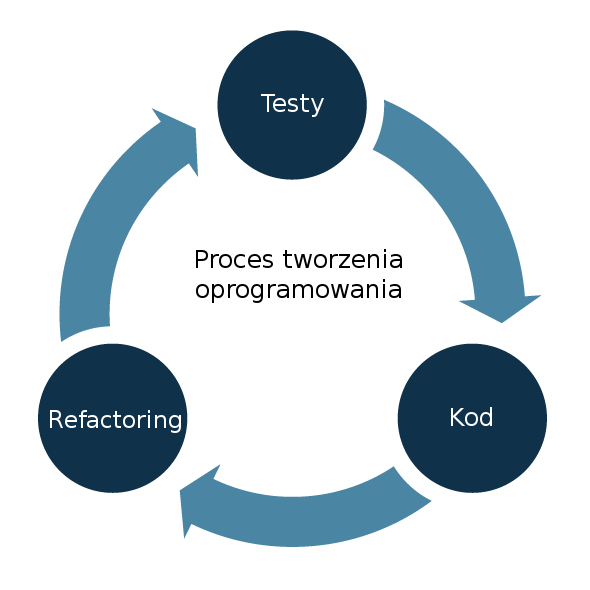
\includegraphics[scale=0.47]{images/test_cycle.png}
          \caption{Schemat postępowania w TDD}
        \end{figure}

      \newpage
      \item Behaviour Driven Development \\
        Technika stworzona przez Dana Northa w 2003 roku. Sam autor powiedział:
        \begin{quote}
          \emph{„Behaviour-driven Development polega na tworzeniu oprogramowania przez opisywanie jego zachowania, z perspektywy jego udziałowców.”}
        \end{quote}

        Wychodzimy naprzeciw klientowi, staramy się go zrozumieć, spełnić jego oczekiwania, aby aplikacja zachowywała się dokładnie tak jak on to sobie wyobraża.

        Tworzy się krótkie historyjki, scenariusze, w których jest opisane jakiego zachowania od aplikacji oczekuje klient. Korzysta się z trzech głównych słów kluczowych:
          \begin{itemize}
            \item Given (\emph{Podane}) - opisuje stan początkowy aplikacji.
            \item When (\emph{Kiedy}) - wszystki kroki jaki klient/użytkownik musi wykonać aby osiągnąć cel funkcjonalności.
            \item Then (\emph{Wtedy}) - stan końcowy aplikacji, czyli oczekiwany efekt po przejściu przez wcześniejsze krok.
          \end{itemize}

        Test driven development to testowanie na poziomie kodu, behaviour driven development to testowanie na poziomie aplikacji. Dlatego jeśli korzysta się z obu technik, zaczyna się od BDD, schodząc coraz ,,niżej'', aż do TDD.
    \end{itemize}

  \subsection{Testy integracyjne}
  \subsection{Testy jednostkowe}
